\documentclass{article}
\usepackage[utf8]{inputenc}
\usepackage[english]{babel}
\usepackage[]{amsthm}
\usepackage[]{amssymb}
\usepackage{amsmath}
\usepackage{gensymb}
\usepackage{blindtext}
\usepackage{geometry}
 \geometry{
 a4paper,
 total={170mm,257mm},
 left=20mm,
 top=20mm,
 }
\usepackage{pgfplots}

\pgfplotsset{width=7cm,compat=1.9}

% We will externalize the figures
\usepgfplotslibrary{external}
\tikzexternalize

\newcommand{\ihat}{\;\hat{\textbf{\i}}}
\newcommand{\jhat}{\;\hat{\textbf{\j}}}
\newcommand{\khat}{\;\hat{\textbf{k}}}
\newcommand{\rvec}{\vec{r}(t)}
\newcommand{\drvec}{\vec{r}\;'(t)}
\newcommand\vv[1]{\langle #1 \rangle}
\newcommand\vc[2]{\vec{#1}(#2)}
\newcommand\vcd[2]{\vec{#1}\;'(#2)}
\newcommand\vcdd[2]{\vec{#1}\;''(#2)}
\newcommand\vcddd[2]{\vec{#1}\;'''(#2)}
\newcommand\mgv[1]{\|#1\|}
\newcommand\mgvv[2]{\sqrt{\left(#1\right)^2 + \left(#2\right)^2}}
\newcommand\mgvvv[3]{\sqrt{\left(#1\right)^2 + \left(#2\right)^2 + \left(#3\right)^2}}
\newcommand\rr{\quad\Rightarrow\quad}

\title{Chapter 13 Section 3 \& 4 Problem Set}
\author{Andry Paez}
\date{}

\begin{document}
\maketitle
\section*{Section 3: Arc Length and Curvature}
\subsection*{Problem 1a}

Use Equation 2 to compute the length of the given line segment.
\[
    \vec{r}(t)  = \langle{3-t, 2t, 4t + 1}\rangle \quad 1 \leq{t} \leq{3}
\]
\centerline{\textbf{Solution}} \\
Let the length of the line segment be 

\begin{align*}
    L = \int_{a}^{b} \sqrt{(\frac{dx}{dt})^2 + (\frac{dy}{dt})^2 + (\frac{dz}{dt})^2} \;dt 
    \Rightarrow L = \int_{a}^{b} \|\vec{r}\;'(t)\| \;dt
\end{align*}

\[
    D: \{\:t \;|\; 1 \leq t \leq 3\:\}
\]

\begin{align*}
    \vec{r}\:'(t)  = \langle{-1, 2, 4}\rangle \Rightarrow
    L &= \int_{1}^{3} \sqrt{(-1)^2 + (2)^2 + (4)^2} dt
      &= \int_{1}^{3} \sqrt{21} dt &= \sqrt{21}t \; \Big|_{1}^{3} = \sqrt{21}(3) - \sqrt{21}(1) = 2\sqrt{21}
\end{align*}

   
\subsection*{Problems 3-7 odd}

Find the length of the curve.

\subsubsection*{3. $\vec{r}\;(t) = \langle{t, 3\cos{t}, 3\sin{t}} \rangle \quad 25 \leq t \leq 5$}
\centerline{\textbf{Solution}} \\

\begin{align*}
    \vec{r}\;'(t) = \langle{1, -3\sin{t}, 3\cos{t}} \rangle \Rightarrow
    L &= \int_{-5}^{5} \sqrt{1^2 + (-3\sin{t})^2 + (3\cos t)^2}\;dt \\
    &= \int_{-5}^{5} \sqrt{1 + 9\sin^2t + 9\cos^2t}\; dt\\ 
    &= \int_{-5}^{5} \sqrt{1 + 9(1)}\; dt \\
    &= \int_{-5}^{5} \sqrt{10}\; dt \\ 
    &= \sqrt{10}t\; \Big|_{-5}^{5} dt = \sqrt{10}(5) - \sqrt{10}(-5) = 10\sqrt{10}
\end{align*}


\[
\]

\subsubsection*{5. $\vec{r}\;(t) = \langle{\sqrt{2}t, e^{t}, e^{-t}} \rangle \quad 0 \leq t \leq 1$}
\centerline{\textbf{Solution}} \\

\begin{align*}
    \vec{r}\; '(t) = \langle{\sqrt{2}, e^{t}, -e^{-t}} \rangle \Rightarrow
    L &= \int_{0}^{1} \sqrt{(\sqrt{2})^2 + (e^{t})^{2} + (-e^{-t})^{2}}\; dt \\
      &= \int_{0}^{1} \sqrt{2 + e^{2t} + e^{-2t}}\; dt \\ 
      &= \int_{0}^{1} \sqrt{(e^{t} + e^{-t})^2}\; dt \\
      &= \int_{0}^{1} e^{t} + e^{-t}\; dt \\
      &= e^{t} - e^{-t}\; \Big|_{0}^{1} = (e^{1} - \frac{1}{e^1}) - (e^{0} - \frac{1}{e^0}) = e - \frac{1}{e} - 1 + 1 = e - \frac{1}{e}
\end{align*}



\subsubsection*{7. $\vec{r}\;(t) = \langle{1, t^2, t^3} \rangle \quad 0 \leq t \leq 1$}
\centerline{\textbf{Solution}} \\

\begin{align*}
    \vec{r}\; '(t) = \langle{0, 2t, 3t^2} \rangle \Rightarrow
    L &= \int_{0}^{1} \sqrt{(0)^2 + (2t)^2 + (3t^2)^2}\; dt \\
      &= \int_{0}^{1} \sqrt{4t^2 + 9t^4}\; dt \\
      &= \int_{0}^{1} \sqrt{t^2(4 + 9t^2)}\; dt \\
      &= \int_{0}^{1} t\sqrt{4 + 9t^2}\; dt \\
\end{align*}
Using u-substitution,
\begin{align*}
    u^2 &= 4 + 9t^2 \\
    2udu &= 18t\; dt \\
    \frac{u\;du}{9} &= t\; dt \\
    \int_{0}^{1} t\sqrt{4 + 9t^2}\; dt &= \int_{0}^{1} u \cdot(\frac{1}{9} u) \; du \\
                    &= \frac{1}{9} \int_{0}^{1} u^2\; du = \frac{1}{9} (\frac{1}{3} u^3) \Big|_{2}^{\sqrt{13}} \\
                    &= \frac{1}{27} (u^3) \Big|_{2}^{\sqrt{13}} = \frac{1}{27} (13^{\frac{3}{2}} - 2^3) = \frac{13\sqrt{13}}{27} - 3
\end{align*}
\subsection*{Problems 19-23 odd}

(a) Find the unit tangent and unit normal vectors $\vec{T}(t)$ and $\vec{N}(t)$. \\
(b) Use Formula 9 to find the curvature.

\subsubsection*{19. $\vec{r}(t) = \langle{t^2,\; \sin{t} - t\cos{t},\; \cos{t} + t\sin{t}} \rangle, \quad t > 0$}
\centerline{\textbf{Solution}}
\intertext{\textbf{a.}} 
\[
    \vec{T}(t) = \frac{\drvec}{\|\drvec\|}   
\]
\begin{align*}
    \drvec &= \langle 2t, \cos t - \cos t + t\sin t, -\sin t + \sin t + t\cos t \rangle = \langle 2t, t\sin t, t\cos t \rangle \\
    \|\drvec\| &= \sqrt{4t^2 + t^2\sin^2t + t^2\cos^2t} = \sqrt{4t^2 + t^2} = \sqrt{5t^2} = \sqrt{5}t \quad [\cos^2t + \sin^2t = 1] \\ 
    \vec{T}(t) &= \frac{\langle 2t, t\sin t, t\cos t \rangle}{\sqrt{5}t} = \frac{1}{\sqrt{5}}\langle 2, \sin t, \cos t \rangle
\end{align*}
\[
    \vec{N}(t) = \frac{\vec{T}\;'(t)}{\|\vec{T}\;'(t)\|}
\]
\begin{align*}
    \vec{T}\;'(t) &= \frac{1}{\sqrt{5}}\langle 0, \cos t, -\sin t \rangle \\
    \|\vec{T}\;'(t)\| &= \frac {1}{\sqrt 5} \sqrt{0^2 + \cos^2t + \sin^2t} = \sqrt{1} = \frac{1}{\sqrt 5} \\
    \vec{N}(t) &= \frac{ \frac{1}{\sqrt{5}} \langle 0, \cos t, -\sin t \rangle}{\frac{1}{\sqrt{5}}} = \langle 0, \cos t, -\sin t \rangle 
\end{align*}
\intertext{\textbf{b}}. 
\begin{align*}
    \kappa(t) &= \frac{\|\vec{T}\;'(t)\|}{\|\drvec\|} = \frac{\frac{1}{\sqrt 5}}{\sqrt 5t} = \frac{1}{5t}
\end{align*}
\subsubsection*{21. $\vec{r}(t) = \langle{t, t^2, 4} \rangle$}
\centerline{\textbf{Solution}}
\intertext{\textbf{a}}. 
\begin{align*}
    \drvec &=  \ihat +  2t\jhat \\ 
    \|\drvec\| &= \sqrt{1^2 + (2t)^2} = \sqrt{1 + 4t^2}  \\
    \vec T (t) &=  \frac{\ihat + 2t\jhat}{\sqrt{1 + 4t^2}} = \frac{1}{\sqrt{1 + 4t^2}}(\ihat + 2t\jhat) \\
    \frac{d}{dt} &= [f(t)\vec u (t)] = f'(t)\vec u (t) + f(t)\vec u \;'(t) \quad [vector\;product\;rule] \\  
    \vec T \;'(t) &= -\frac{4t}{(1+4t^2)^{\frac 3 2}}(\ihat + 2t\jhat) + \frac{1}{(1 + 4t^2)^{\frac 1 2}}(2\jhat) \\
                  &= \frac{1}{(1 + 4t^2)^{\frac 3 2}}\left(-4t(\ihat + 2t\jhat) + (1+4t^2)(2\jhat)\right) = \frac{1}{(1 + 4t^2)^{\frac 3 2}}(-4t\ihat - 8t^2\jhat + 2\jhat + 8t^2\jhat) \\
                  &= \frac{1}{(1 + 4t^2)^{\frac 3 2}}(-4t\ihat + 2\jhat) \\
    \| \vec T \;'(t)\| &= \frac{1}{\left(1+4t^2\right)^{\frac 3 2}}\sqrt{(-4t)^2 + 2^2} = \frac{1}{(1 + 4t^2)^{\frac 3 2}} \sqrt{16t^2 + 4} = \frac{1}{(1 + 4t^2)^{\frac 3 2}}\sqrt{4(4t^2 + 1)} = \frac{2}{(1 + 4t^2)^{\frac 3 2}}\sqrt{1+4t^2} \\
                       &= \frac{2}{1+4t^2} \\
    \vec N (t) &=  \frac{\vec T\;'(t)}{\|\vec T\;'(t)\|} = \frac{1}{(1+4t^2)^{\frac 3 2}}(-4t\ihat + 2\jhat) \; \cdot \; \frac{1+4t^2}{2} = \frac{(1+4t^2)^1}{2(1+4t^2)^{\frac 3 2}}(-4t\ihat + 2\jhat) = \frac{1}{\sqrt{1+4t^2}}(-2t\ihat + \jhat)
\end{align*}
\intertext{\textbf{b}}.
\begin{align*}
    \kappa (t) = \frac{\|\vec T\;'(t)\|}{\|\drvec\|} = \frac{2}{1+4t^2} \;\cdot\; \frac{1}{(1+4t^2)^\frac 1 2} = \frac{2}{(1+4t^2)^{\frac 3 2}}
\end{align*}
\subsubsection*{23. $\vec{r}(t) = \langle{t, \frac{1}{2}t^2, t^2} \rangle$}
\centerline{\textbf{Solution}}
\intertext{\textbf{a}}. 
\begin{align*}
    \drvec &= \langle 1, t, 2t \rangle \rr \|\drvec\| = \sqrt{1^2 + t^2 + (2t)^2} = \sqrt{1 + 5t^2} \\ 
    \vec T(t) &= \frac{\drvec}{\|\drvec\|} = \frac{\langle 1, t, 2t \rangle}{\sqrt{1 + t^2 + 4t^2}} = \frac{1}{\sqrt{1 + 5t^2}}\langle 1, t, 2t \rangle \\
    \frac{d}{dt} &= [f(t)\vec u (t)] = f'(t)\vec u (t) + f(t)\vec u \;'(t) \quad [vector\;product\;rule] \\  
    \vec T\;'(t) &= -\frac{5t}{(1+5t^2)^{\frac 3 2}}\langle 1, t, 2t\rangle + \frac{1}{(1+5t^2)^\frac 1 2}\langle 0, 1, 2 \rangle \\
                 &= \frac{1}{(1+5t^2)^{\frac 3 2}}\left(-5t \langle 1, t, 2t \rangle + (1+5t^2)\langle 0, 1, 2 \rangle\right) \\
                 &= \frac{1}{(1+5t^2)^{\frac 3 2}}\left(\langle -5t, -5t^2, -10t^2 \rangle + \langle 0, 1+5t^2, 2+10t^2 \rangle\right) = \frac{1}{(1+5t^2)^{\frac 3 2}} \langle -5t, 1, 2 \rangle \\
    \|\vec T\;'(t)\| &= \frac{1}{(1+5t^2)^{\frac 3 2}}\sqrt{(-5t)^2 + 1^2 + 2^2} = \frac{1}{(1+5t^2)^{\frac 3 2}}\sqrt{25t^2 + 5} = \frac{1}{(1+5t^2)^{\frac 3 2}}\sqrt{5(5t^2 + 1)} \\
                     &= \frac{\sqrt 5 (1+5t^2)^{\frac 1 2}}{(1+5t^2)^{\frac 3 2}} = \frac{\sqrt 5}{1+5t^2} \\
    \|\vec N(t)\| &=  \frac{\vec T\;'(t)}{\|\vec T\;'(t)\|} = \frac{1}{(1+5t^2)^{\frac 3 2}} \langle -5t, 1, 2 \rangle \; \cdot \; \frac{1+5t^2}{\sqrt 5} = \frac{1}{\sqrt 5\sqrt{1+5t^2}} \langle -5t, 1, 2 \rangle  = \frac{1}{\sqrt{5+25t^2}}\langle -5t, 1, 2 \rangle\\ 
\end{align*}
\intertext{\textbf{b}}.
\begin{align*}
    \kappa(t) = \frac{\|\vec T\;'(t)\|}{\|\drvec\|} = \frac{\sqrt 5}{1+5t^2} \; \cdot \; \frac{1}{\sqrt{1+5t^2}} = \frac{\sqrt 5}{(1+5t^2)^{\frac 3 2}}
\end{align*}
\subsection*{Problem 27}
Use Theorem 10 to find the curvature
\[
    \rvec = \sqrt{6}t^2\ihat + 2t\jhat + 2t^3\khat
\]
\centerline{\textbf{Solution}} \\
Theorem 10 states that $$\kappa(t) = \frac{\|\drvec \times \vec r \;''(t)\|}{\|\drvec\|^3}$$ \\
\begin{align*}
    \vec r \;'(t) &= 2\sqrt 6t \ihat + 2\jhat + 6t^2\khat \rr \vec r \;''(t) = 2\sqrt 6\ihat + 12t\khat \\
    \|\drvec\| &= \sqrt{(2\sqrt 6t)^2 + 2^2 + (6t^2)^2} = \sqrt{24t^2 + 4 + 36t^4} \\ 
               &= \sqrt{4(9t^4 + 6t^2 + 1)} = 2\sqrt{(3t^2 +1)^2} = 2(3t^2+1) \\
\end{align*}

\begin{align*}
    \drvec \times \vec r \;''(t)&  \Rightarrow 
\begin{vmatrix}
    \ihat & \jhat & \khat \\
    \\
    2\sqrt 6t & 2 & 6t^2 \\
    \\
    2\sqrt 6 & 0 & 12t
    \end{vmatrix} \\ 
&= \ihat \begin{vmatrix} 2 & 6t^2 \\\\ 0 & 12t \end{vmatrix} - \jhat \begin{vmatrix} 2\sqrt 6t & 6t^2 \\\\ 2\sqrt 6 & 12t \end{vmatrix} + \khat \begin{vmatrix} 2\sqrt 6t & 2 \\\\ 2\sqrt 6 & 0 \end{vmatrix} \\ 
&= (24t - 0)\ihat - (24t^2\sqrt{6} - 12t^2\sqrt{6})\jhat + (0 - 4\sqrt 6)\khat \\ 
&= 24t\ihat - 12t^2\sqrt 6\jhat - 4\sqrt 6\khat \\
    \| \drvec \times \vec r \;''(t) \| &= \sqrt{ (24t)^2 + (-12t^2\sqrt 6)^2 + (-4\sqrt 6)^2} = \sqrt{576t^2 + 864t^4 + 96} \\ 
                                       &= \sqrt{96(9t^4 + 6t^2 + 1)} = \sqrt{16 \cdot 6(3t^2 + 1)^2} \\
                                       &= 4\sqrt 6(3t^2 + 1) \\
\end{align*}
\begin{align*}
    \kappa(t) &= \frac{\|\drvec \times \vec r \;''(t)\|}{\|\drvec\|^3} = \frac{4\sqrt 6(3t^2 + 1)}{(2(3t^2+1))^3} = \frac{4\sqrt 6(3t^2 + 1)}{8(3t^2+1)^3} = \frac{\sqrt 6}{2(3t^2+1)^2}
\end{align*}
                                             


\begin{align*}
\end{align*}
\subsection*{Problem 28}

Find the curvature of $\rvec = \langle t^2, \ln t, t\ln t \rangle$ at the point $(1, 0, 0)$. \\

\centerline{\textbf{Solution}} \\
\begin{flalign*}
    If \; x &= t^2 \Rightarrow 1 = t^2, \; then \\ 
         t &= 1 ? \Rightarrow \; \ln 1 \equiv 0 \;, \; 1\ln 1 \equiv 0 \\
         \therefore t &= 1\\
\end{flalign*}
\begin{flalign*}
    \drvec &= \langle 2t, \frac 1 t, \ln t + 1 \rangle,\quad \vec r \;''(t) = \langle 2, -\frac{1}{t^2}, \frac 1 t \rangle \\ 
    \vec r \;'(1) &= \langle 2, 1, 1 \rangle, \quad \|\vec r \;'(1)\| = \sqrt{2^2+1^2+1^2}  = \sqrt 6, \quad \vec r \;''(1) = \langle 2, -1, 1 \rangle \\ 
\end{flalign*}
\begin{align*}
    \vec r \;' (1) \times \vec r \;''(1) &\Rightarrow
\begin{vmatrix}
    \ihat & \jhat & \khat \\ 
    \\
    2 & 1 & 1 \\
    \\
    2 & -1 & 1
\end{vmatrix} =
\ihat\begin{vmatrix}1&1\\\\-1&1\end{vmatrix}
- \jhat \begin{vmatrix}2&1\\\\2&1\end{vmatrix}
\khat \begin{vmatrix}2&1\\\\2&-1\end{vmatrix} \\
                      &= (1-(-1))\ihat - (2-2)\jhat + (-2-2)\khat \\ 
                      &= 2\ihat - 4\khat \Rightarrow \langle 2, 0, -4 \rangle \\
\end{align*}
\begin{align*}
    \kappa(1) &= \frac{\| \langle 2, 0, -4 \rangle \|}{\sqrt 6^3} = \frac{\sqrt{2^2 + 0^2 + (-4)^2}}{6^{\frac 3 2}} = \frac{\sqrt 20}{6\sqrt 6} = \frac{2\sqrt 5}{6\sqrt 6} = \frac{\sqrt 5}{3\sqrt 6} = \frac{\sqrt 30}{18} \\
\end{align*}
\subsection*{Problem 31 \& 33}

Use Formula 11 to find the curvature.

\subsubsection*{31. $y = x^4$}
\centerline{\textbf{Solution}} \\
Formula 11 states that 
\[
    \kappa = \frac{|f''(x)|}{[1 + (f'(x)^2)]^{\frac 3 2}}
\]
\begin{align*}
    y &= x^4 \rr y' = 4x^3 \rr y'' = 12x^2 \\
    \kappa &= \frac{|12x^2|}{[1+(4x^3)^2]^{\frac 3 2}} = \frac{12x^2}{(1+16x^6)^{\frac{3}{2}}}
\end{align*}
\subsubsection*{33. $y = xe^x$}
\centerline{\textbf{Solution}} \\
Formula 11 states that 
\[
    \kappa = \frac{|f''(x)|}{[1 + (f'(x)^2)]^{\frac 3 2}}
\]
\begin{align*}
    y' &= e^x + xe^x \rr y'' = e^x + e^x + xe^x = 2e^x + xe^x \\
    \kappa &= \frac {|2e^x + xe^x|} {[1+ (e^x + xe^x)^2]^{\frac 3 2}} = \frac {e^x(2 + x)} {[1+ (e^x + xe^x)^2]^{\frac 3 2}}
\end{align*}
\subsection*{Problem 51}
Find the vectors \textbf{T}, \textbf{N}, and \textbf{B} at the given point.
\[
    \rvec = \langle{t^2, \frac{2}{3}t^3, t}\rangle, \quad (1, \frac{2}{3}, 1)
\]
\centerline{\textbf{Solution}} \\
\[
    \vc T t = \frac{\drvec}{\|\drvec\|}, \quad \vc N t = \frac{\vec T\;'(t)}{\|\vec T\;'(t)\|}, \quad \vc B t = \vc T t \times \vc N t
\]
\[
    z = t \Rightarrow t = 1?, \quad 1^2 \equiv 1,\; \frac 2 3 1^3 \equiv \frac 2 3,\; 1 \equiv 1 \quad \therefore t= 1
\]
\begin{align*}
    \vcd r t &= \vv{2t, 2t^2, 1} \rr \mgv{\vcd r t} = \mgvvv{2t}{2t^2}{1} = \sqrt{4t^2 + 4t^4 + 1} = \sqrt{(2t^2 + 1)^2} = 2t^2 + 1 \\
    \vc T t &= \frac{\vv{2t, 2t^2, 1}}{2t^2+1} \rr \vc T 1 = \vv{\frac 2 3, \frac 2 3, \frac 1 3} \\ 
    \quad f(t) &= \frac{1}{2t^2 + 1}, \; \vec u = \vv{2t, 2t^2, 1} \rr \vcd T t = f\;'(t)\;\vec u + f(t)\;\vec u\;' \\
\end{align*}
\begin{align*}
    \vcd T t &= -4t(2t^2+1)^{-2}\vv{2t,2t^2,1} + (2t^2+1)^{-1}\vv{2,4t,0} \\ 
             &= (2t^2+1)^{-2}(-4t\vv{2t, 2t^2, 1}+(2t^2+1)\vv{2,4t,0}) \\
             &= (2t^2+1)^{-2}(\vv{-8t^2,-8t^3,-4t}+\vv{4t^2+2,8t^3+4t,0}) \\
             &= (2t^2 + 1)^{-2}\vv{-4t^2 + 2, 4t, -4t} \\
             &= 2(2t^2+1)^{-2}\vv{-2t^2+1, 2t, -2t} 
\end{align*}
\begin{align*}
    \vcd T 1 &= 2(2(1)^2+1)^{-2}\vv{-2(1)^2+1, 2(1), -2(1)} = 2(2+1)^{-2}\vv{-2+1, 2, -2} \\ 
             &= \frac 2 9 \vv{-1, 2, -2} = \vv{-\frac{2}{9}, \frac 4 9, -\frac 4 9} \\
    \vc N 1 &= \frac{\vv{-\frac 2 9, \frac 4 9, -\frac 4 9 }}{\mgvvv{-\frac 2 9}{\frac 4 9}{-\frac 4 9}} = \frac{\vv{-\frac 2 9, \frac 4 9, -\frac 4 9 }}{\sqrt{\frac{36}{81}}} \\ 
            &= \frac 9 6\vv{-\frac 2 9, \frac 4 9, -\frac 4 9} = \vv{-\frac 1 3, \frac 2 3, -\frac 2 3}
\end{align*}
\begin{align*}
    \vc B 1 = \vc T 1 \times \vc N 1 =
    \begin{vmatrix}
        \ihat & \jhat & \khat \\ 
        \\
        \frac 2 3 & \frac 2 3 & \frac 1 3 \\ 
        \\
        -\frac 1 3 & \frac 2 3 & -\frac 2 3
    \end{vmatrix} = (-\frac 4 9 - \frac 2 9)\ihat + (-\frac 1 9 + \frac 4 9)\jhat + (\frac 4 9 - (-\frac 2 9))\khat = \vv{-\frac 2 3, \frac 1 3, \frac 2 3}
\end{align*}
\subsection*{Problem 53}

Find equations of the normal plane and osculating plane of the curve at the given point.
\[
    x = \sin{2t},\; y = -\cos{2t},\; z = 4t; \quad (0, 1, 2\pi)
\]

\centerline{\textbf{Solution}} \\
If $z = 4t$ and $z = 2\pi$, then $t = \frac{2\pi}{4} = \frac \pi 2$ \\
$0 \equiv \sin{2(\frac \pi 2)}, \quad 1 \equiv -\cos(2(\frac \pi 2)), \quad 2\pi \equiv 4(\frac \pi 2) \Rightarrow \quad \therefore t = \frac \pi 2$ \\
\\
The point $(0, 1, 2\pi)$ corresponds to $t=\frac \pi 2$

\begin{align*}
\text{Let }\vc r t &= \vv{\sin 2t, -\cos 2t, 4t} \\
    \vcd r t &= \vv{2\cos 2t, 2\sin 2t, 4} \\
    \vcd {r}{\frac \pi 2} &= \vv{-2, 0, 4} \\
\end{align*}
So, the normal plane has normal vector $\vcd {r}{\frac \pi 2} = \vv{-2, 0, 4}$ \\ \\
\\
\intertext{$\therefore$ The equation of the normal plane is}
\begin{align*}
    -2(x-0)+0(y-1)+4(z-2\pi) = 0 \rr -2x + 4z - 8\pi = 0 \quad or \quad 4z - x = 4\pi
\end{align*}

\intertext{To find the osculating plane at $(0, 1, 2\pi)$ we need vectors $\vc T t$ and $\vc N t$}

\begin{align*}
    \vc T t &= \frac{\vcd r t}{\mgv{\vcd r t}} = \frac{\vv{2\cos 2t, 2\sin 2t, 4}}{\sqrt{4\cos^2 2t + 4\sin^2 2t + 16}} = \frac{\vv{2\cos 2t, 2\sin 2t, 4}}{\sqrt{20}} = \frac{1}{2\sqrt 5}\vv{2\cos 2t, 2\sin 2t, 4} \\
            &=  \frac{1}{\sqrt 5}\vv{\cos 2t, \sin 2t, 2} \\ \\
    \vc{T}{\frac \pi 2} &=  \frac{1}{\sqrt 5}\vv{-1, 0, 2} \qquad
    \vcd T t = \frac{1}{\sqrt 5}\vv{-2\sin 2t, 2\cos 2t, 0} \qquad
    \mgv{\vcd{T}{t}} = \frac 1 {\sqrt 5} \sqrt{4\sin^2 2t + 4\cos^2 2t} = \frac{2}{\sqrt 5}
\end{align*}
\begin{align*}
    \vc{N}{\frac \pi 2} &= \frac{\frac{1}{\sqrt 5}\vv{0, -2, 0}}{\frac {2}{\sqrt 5}} = \frac 1 2 \vv {0, -2, 0} = \vv{0. -1. 0}
\end{align*}
A vector normal to the osculating plane would be $\vc B t = \vc T t \times \vc N t \rr \vc{B}{\frac \pi 2} = \vc {T}{\frac \pi 2} \times \vc{N}{\frac \pi 2} \\
= $$\frac{1}{\sqrt 5}$$
\begin {vmatrix} \ihat & \jhat & \khat \\\\
    -1 & 0 & 2 \\\\
    0 & -1 & 0
\end{vmatrix} = $$ \frac {1}{\sqrt 5} \vv{0-(-2), 0-0, 1-0} = \frac{1}{\sqrt 5}\vv{2, 0, 1}$$ \\ \\

$\therefore$ The equation of the osculating plane is
\begin{align*}
    2(x-0)+0(y-1)+1(z-2\pi) = 0 \rr 2x + z - 2\pi = 0 \quad or \quad 2x + z = 2\pi
\end{align*}

\subsection*{Problem 66}

Use Formula 14 to find the torsion at the given value of t.
\[
    \rvec = \langle{\sin{t}, 3t, \cos{t}}\rangle, \quad t = \frac{\pi}{2}
\]
\centerline{\textbf{Solution}} \\
The torsion of a curve with the paramater t is defined as 
\[
    \tau = -\frac{\vcd B t \cdot \vc N t}{\mgv{\vcd r t}}
\]

We need to find $\vc T t$, $\vc N t$, and $\vc B t$ \\
\begin{align*}
    \vc r t = \vv{\sin t, 3t, \cos t } \rr \vcd r t = \vv{\cos t, 3, -\sin t} \rr \mgv{\vcd r t} = \sqrt{\cos^2 t + 9 + \sin^2 t} = \sqrt{10}
\end{align*}
\begin{align*}
    \vc T t &= \frac{\vcd r t}{\mgv{\vc r t}} 
    = \frac{\vv{\cos t, 3, -\sin t}}{\sqrt{10}}
    = \frac{1}{\sqrt{10}}\vv{\cos t, 3, -\sin t}
\end{align*}
\begin{align*}
    \vcd T t &= \frac{1}{\sqrt{10}}\vv{-\sin t, 0, -\cos t} 
    \rr \mgv{\vcd T t} = \frac{1}{\sqrt{10}}\sqrt{\sin^2 t + \cos^2 t} = \frac{1}{\sqrt{10}} \\
    \vc N t &= \frac{\vcd T t}{\mgv{\vcd T t}} = \frac 1 1 \vv{-\sin t, 0, -\cos t} = \vv{-\sin t, 0, -\cos t}
\end{align*}

$\vc B t = \vc T t \times \vc N t = \frac{1}{\sqrt{10}}$
\begin{vmatrix}
    \ihat & \jhat & \khat \\
    \\
    \cos t & 3 & -\sin t \\
    \\
    -\sin t & 0 & -\cos t 
\end{vmatrix}  = $\frac 1 {\sqrt{10}} \vv{-3\cos t - 0, \sin^2 t - (-\cos^2 t), 0 - (-3\sin t)}$ \\

= $\frac 1 {\sqrt{10}} \vv{-3\cos t, 1, 3\sin t}$ \\\\
\begin{align*}
    \vcd B t = \frac 1 {\sqrt{10}} \vv{3\sin t, 0, 3\cos t} \rr \vcd B t \cdot \vc N t &= \frac 1 {\sqrt{10}} \vv{3\sin t, 0, 3\cos t} \cdot \vv{-\sin t, 0, -\cos t} \\ 
                                                                                    &= \frac 1 {\sqrt{10}}(-3\sin^2 t - 3\cos^2 t) = -\frac{3}{\sqrt{10}} \\
\end{align*}

$\therefore$ The torsion of the curve at $t = \frac \pi 2$ is
$$\tau = -\frac{-\frac {3}{\sqrt{10}}}{\sqrt{10}} = \frac {3}{10}$$


\subsection*{Problem 70}

Use Theorem 15 to find the torsion of the given curve at a general point and at the point corresponding to $t = 0$
\[
    \rvec = \langle{\cos{t}, \sin{t}, \sin{t}}\rangle
\]
\centerline{\textbf{Solution}} \\
Theorem 15 states that 
\begin{align*}
    \tau (t) = \frac {[\vcd r t \times \vcdd r t] \cdot \vcddd r t  }{\mgv{\vcd r t \times \vcdd r t}^2}
\end{align*}
\begin{align*}
    \vcd r t = \vv{-\sin t, \cos t, \cos t} \qquad \vcdd r t = \vv{-\cos t, -\sin t, -\sin t} \qquad \vcddd r t = \vv{\sin t, -\cos t, -\cos t} \\
\end{align*}
\begin{align*}
    \vcd r 0 = \vv{0, 1, 1} \qquad \vcdd r 0 = \vv{-1, 0, 0} \qquad \vcddd r 0 = \vv{0, -1, -1} \\
\end{align*}
\begin{align*}

    $[\vcd r 0 \times \vcdd r 0] \cdot \vcddd r 0 = $
    \begin{vmatrix}
        \ihat & \jhat & \khat \\
        \\
        0 & 1 & 1 \\
        \\
        -1 & 0 & 0
    \end{vmatrix}
    $ = \vv{0-0, -1 - 0, 0 -(-1)} = \vv{0, -1, 1}\cdot \vv{0, -1, -1}$ \\
    $ = 0 + 1 - 1 = 0$\\
\\
$\therefore$ The torsion of the curve at $t = 0$ is 
\[
    \tau (0) = \frac{0}{\sqrt{2}^2} = 0
\]

\end{align*}
\section*{Section 4: Motion in Space - Velocity and Acceleration}
\subsection*{Problem 3-7 odd}

Find the velocity, acceleration, and speed of a particle with the given position function. Sketch the path of the particle and draw the velocity and acceleration vectors for the specified value of $t$.

\subsubsection*{3. $\rvec = \langle -\frac 1 2 t^2, t \rangle, \quad t = 2$}
\centerline{\textbf{Solution}} \\
\begin{align*}
    \drvec &= \vec v (t) = \langle -t, 1 \rangle \quad \Rightarrow \quad \vec v (2) = \langle -2, 1 \rangle \\
    \vec r \;''(t) &= \vec a (t) = \langle -1, 0 \rangle \quad\Rightarrow \quad \vec a (2) = \langle -1, 0\rangle \\
    \mgv{\vc v t} &= \sqrt{t^2 + 1}
\end{align*}

\begin{align*}
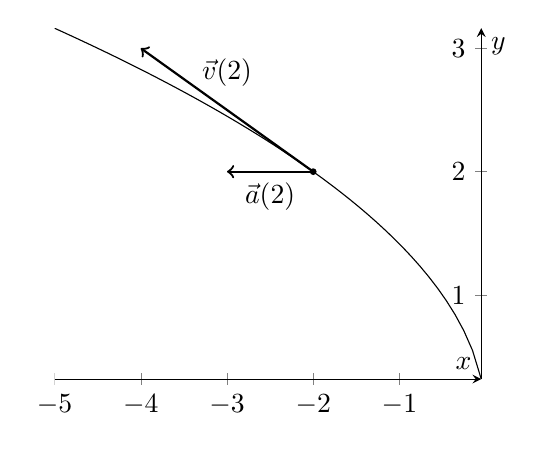
\begin{tikzpicture}
    \begin{axis}[
        axis lines = middle,
        xlabel = \(x\),
        ylabel = {\(y\)},
    ]
    % draw the path
    \addplot[
        color=black,
        samples = 100,
    ]
    {sqrt(-2 * x)}; % function
    % draw the point at t = 2
    \draw[fill=black] (axis cs: -2, 2) circle[radius=1pt];
    % draw the velocity vector at t = 2
    \draw[->, thick] (axis cs: -2, 2) -- (axis cs: -4, 3);
    \node at (axis cs: -3, 2.8) {$\vec v (2)$};
    % draw the acceleration vector at t = 2
    \draw[->, thick] (axis cs: -2, 2) -- (axis cs: -3, 2);
    \node at (axis cs: -2.5, 1.8) {$\vec a (2)$};
    \end{axis}
\end{tikzpicture}
\end{align*}

\subsubsection*{5. $\rvec = 3 \cos t \ihat + 2 \sin t \jhat \quad t = \frac \pi 3 $}

\centerline{\textbf{Solution}} \\
\begin{align*}
    \vcd r t &= \vc v t = \vv{-3\sin t, 2\cos t} \rr \vc v {\frac \pi 3} = \vv{-3(\frac {\sqrt 3} 2), 2(\frac 1 2)} = \vv{-\frac {3\sqrt 3} 2, 1} \\
    \vcdd rt &= \vc a t = \vv{-3\cos t, -2\sin t} \rr  \vc a {\frac \pi 2} = \vv{-3(\frac 1 2), -2(\frac {\sqrt 3} 2)} = \vv{\frac {-3} 2, -\sqrt 3} \\
    \mgv{\vc v t} &= \sqrt{(-3\sin t)^2 + (2\cos t)^2} = \sqrt{9\sin^2 t + 4\cos^2 t} = \sqrt{9(1-\cos^2 t) + 4\cos^2 t} = \sqrt{9 - 5\cos^2 t} \\
\end{align*}
\begin{align*}
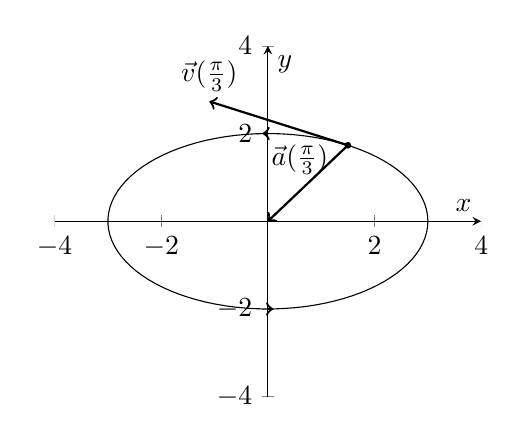
\begin{tikzpicture}
    \begin{axis}[
        axis lines = middle,
        xlabel = \(x\),
        ylabel = \(y\),
        xmin = -4, xmax = 4,
        ymin = -4, ymax = 4,
        clip = false
    ]
    % draw the path
    \addplot[
        color=black,
        samples = 100,
        domain = 0:2*pi
    ]
    ({3 * cos(deg(x))}, {2 * sin(deg(x))}); % parametric function
    % draw the point at t = pi/3 
    \draw[fill=black] (axis cs: 1.5, {sqrt(3)}) circle[radius=1pt];
    % draw the velocity vector at t = pi/3
\draw[->, thick] (axis cs: 1.5, {sqrt(3)}) -- (axis cs: {1.5 - 1.5*sqrt(3)}, {sqrt(3) + 1}) node[above, sloped] {$\vec v (\frac \pi 3)$};
    % draw the acceleration vector at t = pi/3
\draw[->, thick] (axis cs: 1.5, {sqrt(3)}) -- (axis cs: 0, 0);
    \node at (axis cs: 0.6, 1.4) {$\vec a (\frac \pi 3)$};
    % orientation arrows
    \draw[->, thick] (axis cs: 0, 2) -- (axis cs: -0.1, 2);
    \draw[->, thick] (axis cs: 0, -2) -- (axis cs: 0.1, -2);
    \end{axis}
\end{tikzpicture}
\end{align*}

\subsubsection*{7. $\rvec = t\ihat + t^2\jhat + 2\khat \quad t = 1$}
\centerline{\textbf{Solution}} \\
\begin{align*}
    \vcd r t &= \vc v t = \vv{1, 2t, 0} \rr \vc v 1 = \vv{1, 2, 0} \\
    \vcdd r t &= \vc a t = \vv{0, 2, 0} \rr \vc a 1 = \vv{0, 2, 0} \\
    \mgv{\vc v t} &= \sqrt{1^2 + (2t)^2} = \sqrt{1 + 4t^2} \\
\end{align*}

\begin{align*}
\begin{tikzpicture}
    \begin{axis}[
        axis lines = middle,
        xlabel = \(x\),
        ylabel = {\(y\)},
        zlabel = {\(z\)},
        xmin = -4, xmax = 4,
        ymin = -4, ymax = 4,
        zmin = -4, zmax = 4, 
        clip = false,
        view = {110}{30},
        ticks = none
    ]
    % draw the path
    \addplot3[
        surf,
        samples=50,
        domain= -2:2,
    ]
    ({x},{x^2},{2}); % parametric function
    % draw the point at t = 1
    \draw[fill=black] (axis cs: 1, 1, 2) circle[radius=1pt]);
    % draw the velocity vector at t = 1
    \draw[->, thick] (axis cs: 1, 1, 2) -- (axis cs: 2, 3, 2) node[below,sloped] {$\vec v (1)$};
    % draw the acceleration vector at t = 1
    \draw[->, thick] (axis cs: 1, 1, 2) -- (axis cs: 1, 3, 2) node[above, sloped] {$\vec a (1)$};
    \end{axis}
\end{tikzpicture}
\end{align*}

\subsection*{Problems 9-13 odd}
        
Find the velocity, acceleration, and speed of a particle with the given position function.

\subsubsection*{9. $\rvec = \langle t^2+ t, t^2 - t, t^3 \rangle $} 
\centerline{\textbf{Solution}} \\
\begin{align*}
    \vc v t &= \vv{2t + 1, 2t - 1, 3t^2} \\
    \vc a t &= \vv{2, 2, 6t} \\
    \mgv{\vc v t} &= \mgvvv{2t+1}{2t-1}{3t^2} \\ 
                  &= \sqrt {(4t^2 + 4t + 1) + (4t^2-4t + 1) + 9t^4} \\ 
            &= \sqrt{9t^4 +8t^2 + 2}
\end{align*}
\subsubsection*{11. $\rvec = \sqrt 2 t\ihat + e^t\jhat + e^{-t} \khat$}
\centerline{\textbf{Solution}} \\
\begin{align*}
    \vc v t &= \sqrt 2\ihat + e^t\jhat - e^{-t}\khat \\
    \vc a t &= e^t\jhat + e^{-t}\khat \\
    \mgv{\vc v t} &= \mgvvv{\sqrt 2}{e^t}{-e^{-t}} = \sqrt{(e^t + e^{-t})^2} \\ 
                  &= e^t + e^{-t}
\end{align*}
\subsubsection*{13. $\rvec = e^t(\cos t\ihat + \sin t\jhat + t\khat)$}
\centerline{\textbf{Solution}} \\
\begin{align*}
    \vc v t &= e^t(\cos t\ihat + \sin t\jhat + t\khat) + e^t(-\sin t\ihat + \cos t\jhat + \khat)  \\
            &= e^t\left[(\cos t - \sin t)\ihat + (\sin t + \cos t)\jhat + (t + 1)\khat\right] \qquad [\text{vector product rule}] \\
            &= e^t(\cos t - \sin t)\ihat + e^t(\sin t + \cos t)\jhat + e^t(t + 1)\khat \\
    \vc a t &= \left[e^t(\cos t - \sin t) + e^t(-\sin t - \cos t)\right]\ihat + \left[e^t(\sin t + \cos t) + e^t(\cos t - \sin t)\right]\jhat \\
            &+ \left[e^t(t + 1) + e^t\right]\khat \\
            &= e^t(-2\sin t)\ihat + e^t(2\cos t)\jhat + e^t(t + 2)\khat \\
            &= e^t\left[-2\sin t\ihat + 2\cos t\jhat + (t + 2)\khat \right] \\
    \mgv{\vc v t} &= \mgvvv{(e^t) (\cos t - \sin t}{-\sin t - \cos t}{t + 1} \\
                  &= \sqrt{e^{2t}}\sqrt{\cos^2 t - 2\cos t \sin t + \sin^2 t + \sin^2 t + 2\cos t \sin t + \cos^2 t + t^2 + 2t + 1} \\ 
                  &= e^t\sqrt{t^2 + 2t + 3} \\
\end{align*}
\subsection*{Problem 15}

Find the velocity and position vectors of a particle that has the given acceleration and the given initial velocity and position.
\[
    a(t) = 2\ihat + 2t\khat, \quad v(0) = 3\ihat - \jhat, \quad r(0) = \jhat + \khat
\]
\centerline{\textbf{Solution}} \\
\begin{align*}
    \vc v t &= \int \vc a t \; dt  =  \int 2\;dt\ihat + \int 2t\;dt\khat  = (2t + c_1)\ihat + (t^2 + c_2)\khat \\
    \intertext{If $\vc v 0$ = $3\ihat - \jhat$ then}
            &2(0) + c_1 = 3 \rr c_1 = 3, \quad t^2 + c_2 = 0 \rr c_2 = 0 \\
            &\Rightarrow\quad \vc v t = (2t + 3)\ihat - \jhat + t^2\khat
\end{align*}
\begin{align*}
    \vc r t &= \int \vc v t = \int (2t + 3)\;dt\ihat - \int 1\;dt\jhat + \int t^2\;dt\khat = (t^2 + 3t)\ihat - t\jhat + \frac 1 3 t^3\khat \\
    \intertext{If $\vc r 0 = \jhat + \khat$ then}
            &(0^2 + 3(0))\ihat  - 0\jhat + \frac 1 3(0)^3\khat = \jhat + \khat \rr (t^2 + 3t)\ihat + (1 - t)\jhat + (\frac 1 3 t^2 + 1)\khat \\ 
\end{align*}
\subsection*{Problem 17a}

Find the position vector of a particle that has the given acceleration and the specified initial velocity and position.
\[
    a(t) = 2t\ihat + \sin t\jhat + \cos 2t\khat, \quad v(0) = \ihat, \quad r(0) = \jhat
\]
\centerline{\textbf{Solution}} \\
\begin{align*}
    \vc v t &= \int \vc a t = \int 2t\ihat + \sin t\jhat + \cos 2t\khat \;dt = t^2\ihat -\cos t\jhat + \frac 1 2\sin 2t\khat + \vec C \\
    \text{If $\vc v 0 = \ihat$ then} \\
            &0\ihat - \jhat + 0\khat = \ihat \rr \vec C = \ihat + \jhat \rr \vc v t = (t^2 + 1)\ihat + (1 - \cos t)\jhat + \frac 1 2\sin 2t \khat \\
\end{align*}
\begin{align*}
    \vc r t &= \int \vc v t = \int (t^2 + 1)\ihat + (1 - \cos t)\jhat + \left( \frac 1 2 \sin 2t \right)\khat\;dt \\
            &= \left(\frac 1 3 t^3 + t\right)\ihat + \left(t -\sin t\right)\jhat - \left(\frac 1 4 \cos 2t\right)\khat + \vec C \\
            \text{If $\vc r 0 = \jhat$ then} \\
            &  \left(\frac 1 3 0^3 + 0\right)\ihat + \left(0 -\sin 0\right)\jhat - \left(\frac 1 4 \cos 2(0)\right)\khat = \jhat \\
            &\vec C = \jhat - \frac 1 4 \khat \rr \vc r t = \left(\frac 1 3 t^3 + t\right)\ihat + (t - \sin t + 1)\jhat - \left(\frac 1 4 \cos 2t - \frac 1 4\right)\khat
\end{align*}
\subsection*{Problem 23}

A projectile is fired with an initial speed of $200\frac m s$ and angle of elevation $60 \degree$. Find $(a)$ the range of the projectile, $(b)$ the maximum height reached, and $(c)$ the speed at impact.

\centerline{\textbf{Solution}} \\
\begin{align*}
\begin{tikzpicture}
    % diagram of problem 
    \draw (0, 0) -- (4, 0) -- (4, 2) -- (0, 0); 
    \node at (1.5, 1) [left] {$\vec v_0 = 200\frac m s$};
    \node at (1.5, 0.5) [below] {$\theta = 60 \degree$};
    \node at (2, 0) [below] {$\Delta x$}
    \node at (4, 1) [right] {$\Delta y$}
\end{tikzpicture}
\end{align*}
\begin{align*}
    \intertext{\textbf{a.}} 
    \begin{cases}
        \Delta x = v_0 t \cos \theta \\
        \Delta y = v_0 t \sin \theta - \frac 1 2 g t^2
    \end{cases} \rr 
    \begin{cases}
        \Delta x = 100t \\
        \Delta y = 100\sqrt 3 t - 4.9t^2
    \end{cases} \\
    \\
    \intertext{The range of the projectile is the value of $t$ when $y = 0$ (this is when it hits the ground)}
    0 = 100\sqrt 3 t - 4.9t^2 \rr 0 = t(100\sqrt 3 - 4.9t) \rr t = \frac{100\sqrt 3}{4.9} \approx 35.3\:s && \\
    \Delta x = 100(35.3) \approx 3530\:m && \\
\end{align*}
\begin{align*}
    \intertext{\textbf{b.}} 
    \intertext{The maximum height reached is the value of $y$ when $y \;'(t) =  0 \;\text{or}\;\vc {v_y}{t} = 0$ (this is when it's about to switch direction)}
    &\vc {v_y}{t} = 100\sqrt 3 - 9.8t \rr 0 = 100\sqrt 3 - 9.8t \rr t = \frac{100\sqrt 3}{9.8} \approx 17.7\:s \\
    & y_{max} = y(17.7\:s) = 100\sqrt 3(17.7\:s) - 4.9(17.7\:s)^2 \approx 1531\:m
\end{align*}
\begin{align*}
    \intertext{\textbf{c.}} 
    \intertext{The speed at impact is the value of $v$ when $y = 0$ which we have the time as $t \approx 35.3\:s$ (from part a)}
    \vc r t &= \vv{100t, 100\sqrt 3 t - 4.9t^2} \rr \vc v t = \vv{100, 100\sqrt 3 - 9.8t} \\
    \vc v {35.3\:s} &= \vv{100, 100\sqrt 3 - 9.8(35.3)} \approx \vv{100, -172.7} \\
    \text{speed at impact} &= \mgv{\vc v {35.3\:s}} = \mgvv{100}{-172.7} \approx 200\frac m s\\
\end{align*}
\subsection*{Problem 26}

A projectile is fired from a tank with initial speed $400 \frac m s$. Find two angles of elevation that can be used to hit a target $3000m$ away.

\centerline{\textbf{Solution}} \\
\begin{align*}
\begin{tikzpicture}
    % diagram of problem 
    \draw (-4, 0) .. controls (0, 4) .. (4, 0); 
    \draw (-4,0) -- (4, 0);
    \draw[-> ,thick] (-4,0) -- (-2, 2);
    \draw[dashed] (4, 0) -- (4, 3);
    \node at (-3.2, 1) [left] {$\vec v_0 = 400\frac m s$};
    \node at (-3, 0.7) [below] {$\theta = ?$};
    \node at (0, 0) [below] {$\Delta x = 3000m$};
    \node at (4, 1.5) [right] {$\Delta y$};
\end{tikzpicture}
\end{align*}
\begin{align*}
    \intertext{Let the horizontal distance of the projectile be $\Delta x = \displaystyle\frac {\vec{v_0}^2 \sin{2\theta}}{g}$}
    3000\:m &= \frac{(400\:\frac m s)^2 \sin 2\theta}{9.8\:\frac m {s^2}} \\
    \sin 2\theta &= \frac{(3000\:m)(9.8\:\frac{m}{s^2})}{160000\:\frac{m^2}{s^2}} \\
    2\theta &= \frac{\sin^{-1}{(0.18375)}} 2 \\
    2\theta \approx 10.6\degree &\rr 2\theta \approx 169.4\degree \qquad[180\degree - 10.6\degree] \\
    \intertext{$\therefore$ The angles of elevation are $5.3\degree$ and $84.7\degree$}
\end{align*}
\subsection*{Problem 27}

A rifle is fired with angle of elevation $36\degree$. What is the initial speed if the maximum height of the bullet is $1600 ft$?

\centerline{\textbf{Solution}} \\
\begin{align*}
\begin{tikzpicture}
    % diagram of problem 
    \draw (-4, 0) .. controls (0, 4) .. (4, 0); 
    \draw (-4,0) -- (4, 0);
    \draw[-> ,thick] (-4,0) -- (-2, 2);
    \draw[dashed] (0, 0) -- (0, 3);
    \node at (-3.2, 1) [left] {$\vec v_0 = ?$};
    \node at (-2.7, 0.7) [below] {$\theta = 36\degree$};
    \node at (0, 0) [below] {$\Delta x$};
    \node at (0, 1.3) [right] {$y_{max} = 1600ft$}; 
\end{tikzpicture}
\end{align*}
\begin{align*}
    \intertext{The maximum height will be when the velocity in the $y$ direction is 0}
    \vc r t &= (\vec v_0 \cos 36)t \ihat + \left((\vec v_0  \sin 36)t - \frac 1 2 g t^2\right)\jhat \\
    \vc v t &= \vec v_0 \cos 36 \ihat + \left(\vec v_0 \sin 36 - g t\right)\jhat \\
    \intertext{So the maximum height will be when $(\vec v_0 \sin 36) - gt = 0$}
    \vec v_0 \sin 36 &= gt \rr t = \frac{\vec v_0 \sin 36}{g} \\
    \intertext{Substituting this value of $t$ into the $y$ component of the position vector}
    y_{max} &= \left(\vec v_0 \sin 36\right)\left(\frac{\vec v_0 \sin 36}{g}\right) - \frac 1 2 g \left(\frac{\vec v_0 \sin 36}{g}\right)^2 \\ 
    \intertext{Solving for $\vec v_0$}
    1600 &= \left(\vec v_0 \sin 36\right)\left(\frac{\vec v_0 \sin 36}{g}\right) - \frac 1 2 g \left(\frac{\vec v_0 \sin 36}{g}\right)^2 \\
    1600 &= \frac{\vec v_0^2 \sin^2 36}{g} - \frac 1 2 \left(\frac{\vec v_0^2 \sin^2 36}{g}\right) \\
    1600 &= \frac{\vec v_0^2 \sin^2 36}{2g} \rr \vec v_0 = \sqrt{\frac{3200(32\:\frac {ft}{s^2})}{\sin^2 36}} \approx 544\: \frac {ft}{s}\\
    \intertext{$\therefore$ The initial speed of the bullet would be about $544\:\frac {ft}{s}$}
\end{align*}
\subsection*{Problem 37 \& 39}

Find the tangential and normal components of the acceleration vector.

\subsubsection*{37. $\rvec = (t^2 + 1)\ihat + t^3\jhat, \quad t \geq 0    $}
\centerline{\textbf{Solution}} \\
\begin{align*}
    \intertext{Let the tangential component of acceleration be}
    a_T &= \frac {\vc v t \cdot \vc a t}{\mgv{\vc v t}} \\
    \intertext{And the normal component of acceleration}
    a_N &= \frac {\vc v t \times \vc a t}{\mgv{\vc v t}}
    \intertext{First we need to find $\vc v t$, $\vc a t$, $\mgv{\vc v t}$, and $\vc v t \times \vc a t$}
    \vc v t = 2t\ihat + 3t^2\jhat& \rr \vc a t = 2\ihat + 6t\jhat \\
    \mgv{\vc v t}  = \sqrt{4t^2 + 9t^4} = t\sqrt{4 + 9t^2}& \rr \vc v t \times \vc a t \\
    &= \begin{vmatrix}
        \ihat & \jhat & \khat \\
        \\
        2t & 3t^2 & 0 \\
        \\
        2 & 6t & 0
    \end{vmatrix} = (12t^2 - 6t^2)\khat = 6t^2\khat \\
    \intertext{Now we can find the tangential and normal components of acceleration}
    a_T = \frac{2t(2) + 3t^2(6t)}{t\sqrt{4 + 9t^2}} &= \frac{4t + 18t^3}{t\sqrt{4 + 9t^2}} = \frac {4 + 18t^2}{\sqrt{4 + 9t^2}} \\
    a_N = \frac {\sqrt{36t^4}}{t\sqrt{4 + 9t^2}} &= \frac{6t^2}{t\sqrt{4 + 9t^2}} = \frac {6t}{\sqrt{4 + 9t^2}}
\end{align*}
\subsubsection*{39. $\rvec = \cos t\ihat + \sin t\jhat + t\khat$}
\centerline{\textbf{Solution}} \\
\begin{align*}
    \intertext{Let the tangential component of acceleration be}
    a_T = \frac {\vc v t \cdot \vc a t}{\mgv{\vc v t}} \\
    \intertext{And the normal component of acceleration}
    a_N = \frac {\vc v t \times \vc a t}{\mgv{\vc v t}}
    \intertext{First we need to find $\vc v t$, $\vc a t$, $\mgv{\vc v t}$, and $\vc v t \times \vc a t$}
    \vc v t = -\sin t\ihat + \cos t\jhat + \khat& \rr \vc a t = -\cos t\ihat -\sin t\jhat \\
    \mgv{\vc v t} = \sqrt{\sin^2 t + \cos^ t + 1} = \sqrt 2& \rr \vc v t \times \vc a t \\
    &= \begin{vmatrix} 
        \ihat & \jhat & \khat \\
        \\
        -\sin t & \cos t & 1 \\
        \\
        -\cos t & -\sin t & 0 \\
    \end{vmatrix} \\
    &= (0 - (-\sin t))\ihat + (-\cos t - 0)\jhat + (\sin^2 t - (-\cos^2 t))\khat \\
    &= \sin t \ihat -\cos t \jhat + \khat 
    \intertext{Now we can find the tangential and normal components of acceleration}
    a_T &= \frac{(-\sin t)(-\cos t) + (\cos t)(-\sin t)}{\sqrt 2} = \frac{\cos t \sin t - \cos t \sin t}{\sqrt 2} = 0\\
    a_N &= \frac{\sqrt{(\sin t)^2 + (-\cos t)^2 + 1^2}}{\sqrt 2} = \frac{\sqrt 2}{\sqrt 2} = 1
\end{align*}
\subsection*{Problem 41}

Find the tangential and normal components of the acceleration vector at the given point.
\[
    \rvec = \ln t\ihat + (t^2 + 3t)\jhat + 4\sqrt t\khat, \quad (0, 4, 4)
\]
\centerline{\textbf{Solution}} \\
\begin{align*}
    \intertext{Let the tangential component of acceleration be}
    a_T = \frac {\vc v t \cdot \vc a t}{\mgv{\vc v t}} \\
    \intertext{And the normal component of acceleration}
    a_N = \frac {\vc v t \times \vc a t}{\mgv{\vc v t}}
    \intertext{First we need to find which value of $t$ the point $(0, 4, 4)$ corresponds to, $\vc v t$, and $\vc a t$}
    \vc r t = \ln t\ihat + (t^2 + 3t)\jhat + 4\sqrt t\khat& \rr \vc v t = \frac 1 t \ihat + (2t + 3)\jhat + \frac 2 {\sqrt t}\khat \\
    \vc a t &= -\frac 1 {t^2} \ihat + 2\jhat - \frac 1 {\sqrt {t^3}}\khat \\
    \intertext{Since $\ln t = 0$ given by the point $(0, 4, 4)$, then $t$ must be 1}
    \intertext{Then we evaluate $\mgv{\vc v t}$ and $\mgv{\vc v t \times \vc a t}$ at t = 1}
    \mgv{\vc v t} &= \mgvvv{1}{5}{2} = \sqrt{30} \\
    \vc v 1 \times \vc a 1 =
    \begin{vmatrix} 
        \ihat & \jhat & \khat \\
        \\
        1 & 5 & 2 \\ 
        \\
        -1 & 2 & -1 \\
    \end{vmatrix} &= (-5 - 4)\ihat + (-2 - (-1))\jhat + (2 - (-5))\khat \\
    &=  -9\ihat - \jhat + 7\khat 
    \intertext{Now we can find the tangential and normal components of acceleration}
    \vc v 1 = \ihat + 5\jhat + 2\khat& \rr \vc a 1 = -\ihat + 2\jhat -\khat \\
    a_T &= \frac {-1 + 10 -2}{\sqrt{30}} = \frac 7 {\sqrt{30}} \\
    a_N &= \frac {\mgvvv{-9}{-1}{7}}{\sqrt{30}} = \sqrt{\frac {131}{30}}
\end{align*}
\end{document}
